\documentclass[]{article}
\usepackage{lmodern}
\usepackage{amssymb,amsmath}
\usepackage{ifxetex,ifluatex}
\usepackage{fixltx2e} % provides \textsubscript
\ifnum 0\ifxetex 1\fi\ifluatex 1\fi=0 % if pdftex
  \usepackage[T1]{fontenc}
  \usepackage[utf8]{inputenc}
\else % if luatex or xelatex
  \ifxetex
    \usepackage{mathspec}
  \else
    \usepackage{fontspec}
  \fi
  \defaultfontfeatures{Ligatures=TeX,Scale=MatchLowercase}
\fi
% use upquote if available, for straight quotes in verbatim environments
\IfFileExists{upquote.sty}{\usepackage{upquote}}{}
% use microtype if available
\IfFileExists{microtype.sty}{%
\usepackage[]{microtype}
\UseMicrotypeSet[protrusion]{basicmath} % disable protrusion for tt fonts
}{}
\PassOptionsToPackage{hyphens}{url} % url is loaded by hyperref
\usepackage[unicode=true]{hyperref}
\hypersetup{
            pdfborder={0 0 0},
            breaklinks=true}
\urlstyle{same}  % don't use monospace font for urls
\usepackage[margin=1in]{geometry}
\usepackage{graphicx,grffile}
\makeatletter
\def\maxwidth{\ifdim\Gin@nat@width>\linewidth\linewidth\else\Gin@nat@width\fi}
\def\maxheight{\ifdim\Gin@nat@height>\textheight\textheight\else\Gin@nat@height\fi}
\makeatother
% Scale images if necessary, so that they will not overflow the page
% margins by default, and it is still possible to overwrite the defaults
% using explicit options in \includegraphics[width, height, ...]{}
\setkeys{Gin}{width=\maxwidth,height=\maxheight,keepaspectratio}
\IfFileExists{parskip.sty}{%
\usepackage{parskip}
}{% else
\setlength{\parindent}{0pt}
\setlength{\parskip}{6pt plus 2pt minus 1pt}
}
\setlength{\emergencystretch}{3em}  % prevent overfull lines
\providecommand{\tightlist}{%
  \setlength{\itemsep}{0pt}\setlength{\parskip}{0pt}}
\setcounter{secnumdepth}{0}
% Redefines (sub)paragraphs to behave more like sections
\ifx\paragraph\undefined\else
\let\oldparagraph\paragraph
\renewcommand{\paragraph}[1]{\oldparagraph{#1}\mbox{}}
\fi
\ifx\subparagraph\undefined\else
\let\oldsubparagraph\subparagraph
\renewcommand{\subparagraph}[1]{\oldsubparagraph{#1}\mbox{}}
\fi

% set default figure placement to htbp
\makeatletter
\def\fps@figure{htbp}
\makeatother

\usepackage{etoolbox}
\makeatletter
\providecommand{\subtitle}[1]{% add subtitle to \maketitle
  \apptocmd{\@title}{\par {\large #1 \par}}{}{}
}
\makeatother
\usepackage{setspace}\doublespacing
\usepackage{lineno}\linenumbers
% https://github.com/rstudio/rmarkdown/issues/337
\let\rmarkdownfootnote\footnote%
\def\footnote{\protect\rmarkdownfootnote}

% https://github.com/rstudio/rmarkdown/pull/252
\usepackage{titling}
\setlength{\droptitle}{-2em}

\pretitle{\vspace{\droptitle}\centering\huge}
\posttitle{\par}

\preauthor{\centering\large\emph}
\postauthor{\par}

\predate{\centering\large\emph}
\postdate{\par}

\date{}

\begin{document}

\section{A multivariate equivalency and general test for Rensch's Rule:
Implications for the evolution of sexual shape
dimorphism}\label{a-multivariate-equivalency-and-general-test-for-renschs-rule-implications-for-the-evolution-of-sexual-shape-dimorphism}

\hfill\break

\textbf{Keywords}: Sexual dimorphism, multivariate, morphological
evolution \hfill\break

\textbf{Short Title}: Multivariate Test of Rensch's Rule \hfill\break

\section{Abstract}\label{abstract}

Rensch's rule, the allometric association between the degree of sexual
dimorphism and overall body size, is an important framework for
understanding the evolution of trends in phenotypic differentiation
between the sexes across taxa. While virtually all recent treatments
have explored the degree of sexual size dimorphism, understanding how
dimorphism in other phenotypic traits evolves is equally relevant.
Indeed, Rensch's original treatment focused not only on size, but also
on dimorphism in relative body proportions, coloration, the presence of
ornaments, etc. Here, we derive a multivariate equivalency for viewing
trends in sexual dimorphism -- relative to overall body size -- across
taxa, and provide a generalized test to determine whether such patterns
are consistent with Rensch's rule. For univariate linear traits such as
body size, our approach yields equivalent results to those from standard
procedures, but our test is also capable of detecting trends in
multivariate datasets like shape. Computer simulations reveal the method
displays appropriate statistical properties, and an empirical example in
Mediterranean lizards illustrates the efficacy of our approach on both
univariate and multivariate phenotypes. Our generalized procedure
substantially extends the toolkit available for investigating
macroevolutionary patterns of sexual dimorphism and seeking a better
understanding of the processes that underlie them.

\newpage

\section{Introduction}\label{introduction}

It is widely observed that males and females of the same species are not
identical, but rather differ -- sometimes substantially -- in their
phenotypic characteristics (Fairbairn 1997, 2013). Indeed, sexual
dimorphism is pervasive across many animal clades, and understanding the
causes for these patterns has attracted considerable attention in
evolutionary biology for well over a century (e.g., Darwin 1871;
Fairbairn et al. 2007). One of the most conspicuous differences between
males and females is in their body sizes (Andersson 1994), where
sex-specific differences are often hypothesized to be the result of
selection pressures related to reproduction, or the distinct ecological
roles of males and females in their respective habitat (Cox et al. 2003;
Stephens and Wiens 2009; Kaliontzopoulou et al. 2015; Tarr et al. 2018;
Littleford-Colquhoun et al. 2019). For example, both sexual selection on
male body size (Cox et al. 2003; Garcia-Navas et al. 2015; Horne et al.
2020), and fecundity selection on female body size (Serrano-Meneses and
Szekely 2006; Stuart-Fox 2008), are expected to enhance the degree of
sexual size dimorphism in taxa over evolutionary time. Likewise, when
males and females respond differently to environmental factors,
intraspecific competition may generate ecological divergence between
them, resulting in varying patterns of sexual dimorphism (Butler et al.
2000; Bolnick and Doebeli 2003; Dayan and Simberloff 2005;
Kaliontzopoulou et al. 2010; Meiri et al. 2014). \hfill\break

At macroevolutionary scales, changes in the relative contribution of the
selective forces above may create variation in the degree of sexual
dimorphism displayed across closely related taxa. For instance, sister
species inhabiting different environments, or possessing distinct
ecological adaptations, may exhibit differing degrees of sexual
dimorphism, as a result of the varying intensity of sexual selection
they endure (Östman and Stuart-Fox 2011). Likewise, the interplay
between sexual and natural selection that species experience may result
in sexual dimorphism of differing magnitudes across taxa (Blanckenhorn
et al. 2006; Stuart-Fox and Moussalli 2007; Kaliontzopoulou et al.
2015). One evolutionary framework that connects adaptive explanations
for the evolution of sexual size dimorphism (SSD) with trends in overall
body size across taxa is Rensch's rule. Here it is predicted that SSD
will increase with species' average body size in species where males are
the larger sex (hyperallometry), and likewise will decrease with
increasing body size where females are the larger sex (hypoallometry)
(Abouheif and Fairbairn 1997; Fairbairn 1997). Put another way, Rensch's
rule predicts that the extent of sexual dimorphism increases at more
extreme body sizes (both large and small) across taxa. Empirical studies
have documented trends in SSD consistent with Rensch's rule in a wide
variety of animal taxa (Dale et al. 2007; Ceballos et al. 2013; Regis
and Meik 2017; Johnson et al. 2017). However, other clades display the
converse trend (Burbrink and Futterman 2019; Peñalver-Alcázar et al.
2019), and some clades display no relationship between SSD and body size
(Astúa 2010; Hirst and Kiørboe 2014; Johnson et al. 2017). From an
evolutionary perspective, the association between SSD and body size has
been hypothesized to be driven by variation in ontogenetic or static
allometries across taxa, which results from the influence of sexual
selection on growth and maturation patterns (Rensch 1960; Dale et al.
2007). \hfill\break

Interestingly, virtually all evaluations of Rensch's rule have
investigated patterns of sexual size dimorphism, yet Rensch's original
contributions were concerned with a much wider array of phenotypic
traits that can differ between the sexes. These included not only sexual
differences in body size, but also in general body proportions (e.g.,
relative wing and limb lengths), the degree of complexity of different
body structures, the presence of sex-specific ornamentation (e.g.,
horns, body coloration, etc.), and other sex-specific differences
(Rensch 1950, 1960). In like manner, some studies have documented
patterns of sexual shape dimorphism (e.g., Berns and Adams 2013; Kelly
et al. 2013; Kaliontzopoulou et al. 2015), sex-specific differences in
ornamentation (Geist and Bayer 1988; Emlen 2008; Watson and Simmons
2010), or coloration (e.g., Endler 1983). However, such studies have
typically been restricted to one or a few taxa, and have not explained
macroevolutionary variation in sexual dimorphism in a manner that
relates directly to Rensch's rule. Thus, when viewed from this
perspective, Rensch's (1950) vision was far more synthetic, as he sought
to explain the extent to which sexual dimorphism -- across a general
suite of phenotypic characteristics -- scaled with overall body size in
organisms, and why some species displayed a greater degree of sexual
dimorphism than did others. Remarkably, patterns of intraspecific static
allometry in sexually selected traits establishes a direct link between
variation in those traits relative to size, and the evolutionary
allometry across taxa in the degree of sexual dimorphism that may be
expected (see also Rensch 1960; Reiss 1986; Bonduriansky 2007). Under
this framework, the ``exaggeration'' of body structures or other
phenotypic traits with increasing body size is predicted to translate,
at macroevolutionary scales, into increased degrees of sexual dimorphism
with increasing body size. However, despite this clear prediction, and
Rensch's original observations, the evolutionary scaling of the degree
of sexual dimorphism in phenotypic traits other than size, remains
largely unexplored. \hfill\break

Another current limitation in our understanding of Rensch's rule is the
fact that to date, all studies have been conducted exclusively on
univariate data, primarily regarding body size. However, understanding
phenotypic evolution is inherently a multivariate endeavor (Blows 2007;
Collyer et al. 2015; Adams and Collyer 2018, 2019), as processes such as
natural and sexual selection simultaneously operate on more than one
trait (Lande 1979; Lande and Arnold 1983), and can affect variation in
complex multidimensional traits such as shape. To interrogate such
patterns, the analytics used to evaluate evolutionary trends in
phenotypic datasets must be sufficiently general to accommodate this
empirical fact. Unfortunately, all current analytical approaches for
evaluating trends in sexual dimorphism as they relate to overall body
size are explicitly univariate; thereby excluding the possibility of
evaluating patterns in complex multidimensional traits such as
organismal shape. Though is has been extensively documented in sexual
size dimorphism, it remains unknown whether Rensch's rule applies
equally to sexual shape dimorphism, as determining this requires an
analytical framework capable of evaluating trends in sexual dimorphism
in both univariate and multivariate datasets. \hfill\break

In this paper, we derive a multivariate equivalency for inspecting
variation in sexual dimorphism -- relative to overall body size --
across taxa, and provide a generalized test to determine whether they
are consistent with Rensch's rule. Our procedure is appropriate for
evaluating trends in univariate traits measured on a linear scale (such
as body size or relative limb length), as well as in multivariate
datasets representing complex phenotypes (such as sets of body
proportions or landmark-based shape data). For univariate data, the
approach yields equivalent results to what is normally accomplished for
size-based SSD evaluations. However, the approach extends these
procedures for the examination of sexual dimorphism in multivariate
data, thereby increasing the potential for our conceptual understanding
of the consequences of sexual and natural selection on complex
organismal phenotypes. We conduct a series of computer simulations
demonstrating that the approach displays appropriate statistical
properties when evaluating trends in both univariate and multivariate
data. We also provide an empirical example in Mediterranean green
lizards which illustrates the efficacy of our approach on both
univariate and multivariate datasets. Finally, we highlight the new
avenues of evolutionary research that our generalization facilitates,
and make comments on the prospects for future empirical advances.

\section{Methods and Results}\label{methods-and-results}

\subsection{\texorpdfstring{\emph{Conceptual
Development}}{Conceptual Development}}\label{conceptual-development}

To arrive at a general test for Rensch's rule that can accommodate
multivariate data, we must first derive a series of mathematical
equivalencies based upon how interspecific patterns of size dimorphism
are typically evaluated. For sexual size dimorphism, interspecific
patterns are often inspected using a bivariate plot, where the size of
one sex is plotted against the size of the other sex (e.g., Fairbairn
and Preziosi 1994; Abouheif and Fairbairn 1997; Ceballos et al. 2013).
An idealized example is shown in Fig. 1A, with male size plotted against
female size. The diagonal line represents no size dimorphism; or a 1:1
size ratio between the sexes across the range of body sizes for species
in the clade of interest. In this construction (i.e., with females
plotted on the x-axis), deviations from this line represent differential
trends in size dimorphism across taxa. To evaluate such patterns
statistically, a phylogenetic regression is performed, and in this case,
a slope significantly greater than 1.0 (i.e., \(\beta_{1}>1.0\)) would
be treated as evidence that the evolutionary changes in sexual size
dimorphism across taxa are consistent with Rensch's rule (Fairbairn
1997). \hfill\break

An equivalent representation of patterns of sexual dimorphism may also
be found using ratios (e.g., male size:female size). When plotted
against the average size for each species (Fig. 1B), the same
information is conveyed as is found in the more commonly utilized male -
female plot of Fig. 1A. However, in this representation, the line
designating no sexual dimorphism is horizontal, with a slope of zero
(i.e., \(\beta_{1}=0.0\)) and an intercept of 1.0. As before, a
phylogenetic regression may be performed on these data, and in this
case, if the slope is significantly steeper than zero (i.e.,
\(\beta_{1}>0.0\)), patterns consistent with Rensch's rule are observed.
\hfill\break

A third equivalency is shown in Fig. 1C. Here, the Euclidean distance
between male and female means for each species
(\(D_{SD}=\sqrt{(Y_{male}-Y_{female})^2}\)) is shown relative to the
overall size of the species. This plot is similar to a Bland-Altmann
plot (Altman and Bland 1983), except that the Euclidean distance, rather
than a difference score, is plotted along the y-axis (as distances can
accommodate data of different dimensionality). Under Rensch's rule, this
\emph{sexual dimorphism distance} may become greater as species are
progressively larger (hyperallometry, sensu Abouheif and Fairbairn 1997)
or may become greater as species are progressively smaller
(hypoallometry, sensu Abouheif and Fairbairn 1997). In both cases,
patterns correspond to species displaying progressively more sexual
dimorphism at extreme body sizes; a trend consistent with Rensch's rule.
Note that the inflection point in Fig. 1C represents an intermediate
size where there is no sexual dimorphism for the trait, and corresponds
to where the male-female regression line of Fig. 1A crosses the line
representing no sexual dimorphism. This inflection point may represent
the overall mean size across species in the lineage, or may be some
other value. For instance, in some lineages (e.g., turtles: Ceballos et
al. 2013), nearly all species are female biased, in which case the
inflection point for \(D_{SD}\) vs.~size would be found at the far-right
end of the plot. \hfill\break

Finally, from \(D_{SD}\) a \emph{sexual dimorphism distance index}
(\(SDDI\)) may be constructed as:

\[SDDI=-1*D_{SD}\] \[SDDI=+1*D_{SD}\]

Here, \(D_{SD}\) is multiplied by either a +1 or -1, based on a
comparison of male and female trait values for the species. For
instance, when single-valued traits on a linear scale are examined
(e.g., leg length or wing extent), \(D_{SD}\) is multiplied by -1 for
those species where females display larger values than males, and
remains unchanged for species where males are larger than females. This
logic is analogous to that of Lovich and Gibbons (1992) for their index
of overall body size dimorphism. However, from a geometric perspective,
this procedure is tantamount to determining which species in Fig. 1A are
found below the 1:1 size line (i.e., the line representing no size
dimorphism), and multiplying those species' \(D_{SD}\) by -1.
\hfill\break

Unfortunately, applying the same logic to multidimensional trait data is
more complicated, as sex-specific differences are not always guaranteed
to align with some \emph{a priori} direction in the multivariate
dataspace. Thus, for multivariate datasets, one of two procedures may be
used. First, for multivariate sets of traits that are measured on the
same linear scale (e.g., length, width, and height measures), one could
envision a hyperdimensional version of the plot displayed in Fig. 1A,
but where the set of male traits are plotted against the set of female
traits. In this construction, because the traits are quantified on the
same measured scale, the 1:1 size vector representing no sexual
dimorphism does exist, and emanates from the origin of the space
extending in a positive direction as the trait values increase. To
determine whether male trait values deviate more from this vector than
do female trait values, a partial least squares analysis may be
performed (Rohlf and Corti 2000). Partial least squares (PLS) is a
multivariate association procedure which describes the covariation
between sets of traits (in this case, between the set of male traits and
the set of female traits). Scores along the first PLS axis represent the
maximal covariation between male and female traits projected to a single
dimension, and species whose male and female PLS scores are identical
are those displaying no sexual dimorphism. Thus, deviations from that
pattern represent instances of multivariate sexual dimorphism. By
plotting these scores, one may determine which species display female
scores (on \(PLS_1\)) that are larger than their corresponding male
scores (when negative values on \(PLS_1\) correspond to smaller
individuals; otherwise, the converse comparison is used). The \(D_{SD}\)
for these species may then be multiplied by -1 to obtain the \(SDDI\)
for that species. Note that when PLS is used on univariate data, this
procedure obtains values identical to those from the method described
previously where male and female sizes are compared directly. Thus, for
multivariate traits measured on a linear scale, this is a direct
generalization of the standard univariate procedure (see empirical
example below). \hfill\break

Alternatively, one might be interested in examining multidimensional
traits other than linear biometric measurements, such as color or shape.
For instance, one may characterize the shape of males and females using
geometric morphometric methods (Bookstein 1991; Mitteroecker and Gunz
2009; Adams et al. 2013), where the locations of anatomical landmarks
and semilandmarks are used to obtain a set of shape variables. Geometric
morphometric methods also result in a multidimensional characterization
of phenotypic traits, from which the degree of sexual dimorphism for
each species may be quantified using \(D_{SD}\). However, because the
resulting shape variables do not have a one to one correspondence with
linear size measures, there is no \emph{a priori} direction in the
multivariate shape space that is equivalent to the 1:1 size vector found
with sets of linear traits. In fact, for the case of isometry (i.e.,
shape does not change as size changes), all observations are represented
by a single location in the shape space. Thus, while a PLS of male
shapes versus female shapes will describe the covariation between them,
this direction is not guaranteed to align with size, because there is no
direction in the shape space that may be used to unambiguously determine
whether dimorphism is male- or female-biased, as for shape variables
there is no \emph{a priori} directionality. Nonetheless, one may still
quantitatively determine whether the degree of sexual shape dimorphism
covaries with overall body size, by using the sexual dimorphism index as
defined by the dimorphism distance (i.e., \(SDDI=D_{SD}\)) to represent
the degree of multivariate shape dimorphism for each species.
\hfill\break

Once the sexual dimorphism distance index (\(SDDI\)) is calculated, it
may be evaluated against the average size of each species. Here, data
conforming to Rensch's rule will result in significant trends of sexual
dimorphism relative to mean body size (Fig. 1D). As with size ratios,
the line of no sexual dimorphism is a horizontal line, but this time it
is centered on zero, as a distance of zero corresponds to no sexual
dimorphism. Thus, a phylogenetic regression of these data whose slope is
significantly different from zero (e.g., \(\beta_{1}\neq0.0\)) provides
evidence that the evolution of sexual dimorphism is consistent with
patterns expected under Rensch's rule. For cases where traits are
measured on a linear scale, patterns expected under Rensch's rule
exhibit a slope significantly greater than zero (\(\beta_{1}>0.0\)), as
in the usual formulation. Likewise, when using geometric morphometric
shape data (or any other type of mean-centered multidimensional data),
hyperallometric patterns consistent with Rensch's rule would also
display a slope significantly greater than zero (\(\beta_{1}>0.0\)),
indicating that the degree of sexual shape dimorphism increases with
increasing body size. Conversely however, hypoallometric patterns would
display the opposite pattern (\(\beta_{1}<0.0\)), indicating that
smaller species display greater sexual shape dimorphism. \hfill\break

\subsection{\texorpdfstring{\emph{Simulations}}{Simulations}}\label{simulations}

To ascertain the statistical performance of the approach proposed here,
we conducted a series of computer simulations. We evaluated the ability
of SDDI to characterize patterns of sexual dimorphism in both univariate
and multivariate datasets. For each simulation, we generated a
pure-birth phylogeny containing 50 species, on which we simulated
datasets under a Brownian motion model of evolution. For univariate data
(\(p=1\)), a single trait was evolved along the phylogeny, and
represented the female trait values (\(x\)). Next, male values (\(y\))
were simulated in such a manner as to generate a known male:female
relationship (plus random error), using the function:
\(y=\alpha{x}+\mathcal{N}(\mu=0,\sigma=0.1)\). For type I error
simulations, no sexual dimorphism was generated, meaning that the slope,
\(\alpha\), characterized a 1:1 relationship between male and female
trait values (i.e., \(\alpha=1.0\)). For power simulations, we simulated
male values with a slope greater than 1.0 to correspond with patterns
following Rensch's rule (i.e., \(\alpha=1.1\)). A total of 1,000
datasets were generated under each simulation condition. We then
evaluated all datasets using standard approaches (i.e., a phylogenetic
regression of male values versus female values), as well as a
phylogenetic regression of SDDI versus average body size. The proportion
of significant datasets was treated as the type I error (\(\alpha=1.0\))
or power (\(\alpha=1.1\)) respectively. \hfill\break

For multivariate data (\(p=5\)), a slightly different procedure was
utilized. First, average body size (\(s\)) was evolved along the
phylogeny under Brownian motion. Next, female traits (\(\mathbf{X}\))
were simulated on the phylogeny under Brownian motion, using a
\(p\times{p}\) trait covariance matrix with correlations between traits
of (\(r=0.7\)). For simulations where there was no pattern of sexual
dimorphism across species (i.e., type I error simulations) male trait
values were then generated by incorporating random error to the female
trait values, in a manner analogous to that achieved in the univariate
simulations:
\(\mathbf{Y}=\mathbf{X}_{F}+\mathcal{N}(\mu=0,\sigma=0.1\)). For
simulations where patterns of sexual dimorphism covaried with body size
(i.e., power simulations), male trait values were generated by
incorporating random error to the female trait values, but with the
addition that female trait values were pre-multiplied by a scalar value
of body size:
\(\mathbf{Y}=(0.1*s)*\mathbf{X}_{F}+\mathcal{N}(\mu=0,\sigma=0.1\)).
This ensured that male and female trait values covaried with one another
as expected, and also covaried with size in the desired direction. As
before, a total of 1,000 datasets were generated under each simulation
condition. We then evaluated all datasets using a phylogenetic
regression of SDDI versus average body size. The proportion of
significant datasets was treated as the type I error (\(\alpha=1.0\)) or
power (\(\alpha=1.1\)) respectively. \hfill\break

\emph{Simulation Results}: For the univariate dataset, we found that
both a phylogenetic regression of male size on female size, as well as a
phylogenetic regression of \(SDDI\) on body size, resulted in
appropriate type I error rates near the nominal \(\alpha\approx0.05\)
(Fig. 2). Further, when data were simulated under conditions consistent
with Rensch's rule, both procedures were capable of detecting the signal
of the pattern, and did so with very high power. Thus, using the
\(SDDI\) approach proposed here was equivalent to what is normally
utilized for univariate datasets. Likewise, for multivariate data, the
\(SDDI\) approach displayed appropriate type I error
(\(\alpha\approx0.05\)) and high statistical power under the conditions
simulated (Fig. 2). Additionally, multiplying \(D_{SD}\) by \(\pm1\) had
little effect on the outcome for multivariate data, as in both cases
type I error and power results were virtually identical. Thus, methods
for evaluating sexual dimorphism using geometric morphometric data are
anticipated to remain robust. Overall results from these simulations
imply that using the sexual dimorphism distance index (\(SDDI\))
proposed here provides an appropriate means of characterizing patterns
of sexual dimorphism in both univariate and multivariate traits, and
that the procedure is capable of detecting patterns consistent with
Rensch's rule when they are present in phenotypic datasets. \hfill\break

\subsection{\texorpdfstring{\emph{Empirical
Example}}{Empirical Example}}\label{empirical-example}

To illustrate the utility of the approach presented here, we conducted
an analysis of both size and shape dimorphism in a group of
Mediterranean lizards with extensive body size variation. Our dataset
consisted of three data types: male and female values of body size
(snout-vent length: SVL), male and female values for a series of head
measurements (head length, head width, head height, pileus length, and
mouth opening: Fig. 3A), and male and female values of head shape (Fig.
3B). A total of 374 specimens from 21 lineages of green lizards, a
monophyletic clade that includes two genera (\emph{Lacerta} and
\emph{Timon}), were obtained from natural history museum collections.
For each lineage, we obtained samples distributed across the entire
distribution range, resulting in an initial database of 1062 specimens.
In order to take sampling bias into account, we selected the 10 largest
individuals per sex, when sufficient specimens were available, for use
in subsequent size and shape analyses. A detailed account of the
specimens used for this study is available in the Supplemental Material.
\hfill\break

From these specimens, we calculated mean body size for each sex and
lineage. Likewise, we calculated the mean trait values for each sex and
lineage for the set of linear measures. These values were then
standardized by SVL; resulting in a set of head measurements
proportional to body size for each sex \(\times\) lineage combination.
Additionally, we quantified lateral head shape variation using geometric
morphometric methods (Adams et al. 2013). This was accomplished by first
digitizing 17 landmarks and semilandmarks from images of the right side
of the head (Fig. 3B). The thin-plate spline was used to estimate the
position of missing landmarks (Gunz et al. 2009), and the position of
the jaw relative to the skull was standardized using the fixed angle
method (Adams 1999). Next, a generalized Procrustes analysis (Rohlf and
Slice 1990) was performed to eliminate non-shape variation from the
landmark data and align the specimens to a common coordinate system. The
position of semilandmarks (i.e.~11-16, Fig. 3B) was optimized by
minimizing the bending energy (Bookstein 1997). From the aligned
Procrustes coordinates the mean head shape for males and for females was
then calculated for each lineage. Finally, the phylogenetic
relationships among lineages were estimated using published sequences on
five mitochondrial and four nuclear gene fragments, totaling 8383 bp.
These were then used following standard phylogenetic inference
procedures to generate a dated consensus phylogeny for the lineages of
interest (for details see Supplemental Material). \hfill\break

Using these data, we conducted a series of analyses to investigate
whether patterns of sexual size dimorphism (SSD) and sexual shape
dimorphism (SShD) in this group corresponded to expectations under
Rensch's rule. First, we examined patterns of SSD using a phylogenetic
regression of male size against female size. Here, a slope significantly
greater than 1.0 (\(\beta>1.0\)) was treated as evidence consistent with
Rensch's rule. Additionally, we evaluated SSD patterns using the
approach developed here, via a phylogenetic regression of the sexual
size dimorphism index against mean body size for each species. Second,
we evaluated multivariate patterns of sexual dimorphism in head
proportions in relation to body size, using the sexual dimorphism index
obtained from the Euclidean distance between male and female means from
each species (\(D_{SD}\)). Partial least squares was used to determine
which species displayed female scores (on \(PLS_1\)) larger than their
corresponding male scores, and the sexual dimorphism index was then
obtained by multiplying the sexual dimorphism distance by +1 or -1,
respectively (i.e., \(SDDI=\pm1*D_{SD}\)). We then performed a
phylogenetic regression of \(SDDI\) for head proportions versus mean
body size to determine whether patterns of dimorphism corresponded to
what is expected under Rensch's rule. Third, we obtained the degree of
sexual dimorphism in head shape for each species using the Procrustes
distance between male and female means, and from this calculated the
sexual shape dimorphism index (\(SShDI\)) in their original units as
described above (i.e., \(SShDI=D_{SD}\)). We then performed a
phylogenetic regression of sexual shape dimorphism (\(SShDI\)) against
the mean body size for each species to determine whether patterns of
head shape dimorphism were consistent with predictions from Rensch's
rule. Additionally, patterns of head shape dimorphism were further
investigated using principal components analysis of the set of mean male
and female head shapes across species. Finally, we used phylogenetic
correlation (phylogenetic partial least squares: sensu Adams and Felice
2014) to determine whether the degree of head shape dimorphism was
associated with levels of size dimorphism. All analyses were performed
in R 3.6.2 (R Core Team 2019) using the packages \texttt{geomorph}
(Adams and Otárola-Castillo 2013; Adams et al. 2019), \texttt{RRPP}
(Collyer and Adams 2018), and routines written by the authors.
\hfill\break

\emph{Empirical Results}: Using phylogenetic regression, we found a
significant relationship between male size and female size, with a slope
significantly greater than one (\(\beta = 1.39\), \(T=2.91\),
\(P = 0.009\): Fig. 3C). This indicated that the degree of sexual size
dimorphism differed systematically with overall body size; a pattern
consistent with that expected under Rensch's rule. In this case, both
hypoallometry and hyperallometry (\emph{sensu} Abouheif and Fairbairn
1997) were displayed (Fig. 3C). Specifically, in male-biased species,
the degree of sexual dimorphism was greater with increasing body size,
and in female-biased species the degree of sexual dimorphism increased
in smaller species (though the pattern was more pronounced in
male-biased species). Similarly, when using the sexual size dimorphism
index (SSDI), we found a significant and positive evolutionary
relationship between SSDI and mean body size, confirming the Rensch's
rule pattern identified using the commonly-used procedure
(\(\beta = 0.43\), \(F=22.95\), \(Z=1.89\), \(P = 0.004\): Fig. 3D).
\hfill\break

When multivariate patterns of sexual dimorphism were evaluated, we found
that the degree of dimorphism in head proportions increased as body size
increased: a pattern consistent with Rensch's rule (\(F=7.20\),
\(Z=1.41\), \(P = 0.022\): Fig. 3E). Likewise, when patterns of head
shape dimorphism were examined, we found that the degree of sexual shape
dimorphism (SShDI) increased in larger species, and a phylogenetic
regression of sexual shape dimorphism versus mean body size was found to
be significant (\(F=6.05\), \(Z=1.35\), \(P = 0.03\): Fig. 3F). Thus,
for both multivariate datasets, the degree of sexual dimorphism was
enhanced in larger species (hyperallometry; sensu Abouheif and Fairbairn
1997): a pattern consistent with what was expected under Rensch's rule.
To our knowledge, this is the first empirical demonstration of a pattern
following Rensch's rule in multivariate data. \hfill\break

Visualizing patterns of head shape dimorphism using principal components
analysis (Fig. 4), it was evident that males and females occupied
distinct regions of morphospace. Further, the head shapes of males and
females of the smallest lineage, \emph{Lacerta agilis bosnica}, were
distinct from those of the largest species, \emph{Timon lepidus}. When
connected, the sexual shape dimorphism vectors for these two species did
not coincide with one another in the ordination, implying a difference
in sexual shape dimorphism across species. Specifically, the vector for
\emph{T. lepidus} was longer than that for \emph{L. agilis bosnica},
which reflected the greater degree of sexual shape dimorphism exhibited
by this species. Thin-plate spline deformation grids facilitated a
graphical description of these shape differences, where sexual shape
dimorphism in \emph{L. agilis bosnica} was best described as a contrast
between longer-headed males, with an amplified tympanic area; and
short-headed females, with a relatively more reduced tympanic region
(Fig. 4, left). By contrast, sexual shape dimorphism in \emph{T.
lepidus} was both more prominent in the tympanic area, similarly to what
was observed in \emph{L. agilis bosnica}; and also included a
modification of the relative lower jaw area. Indeed, males of \emph{T.
lepidus} were characterized by both a longer posterior head region and
by deeper lower jaw configurations as compared to females of the same
species. \hfill\break

Finally, across taxa, the degree of body size and head shape dimorphism
were significantly correlated with one another (\(r=0.73\),
\(p=0.0001\)), but not when evaluated in a phylogenetic context
(\(r_{PPLS} = 0.361\), \(Z=1.28\), \(P = 0.12\)). Part of this
difference may be explained by the fact that the largest species
(i.e.~members of the genus \emph{Timon}) - which displayed the greatest
degree of both size and shape dimorphism - form a clade within the
broader phylogeny for the group (Fig. 5). Thus, despite the strong
association of size and shape dimorphism, there were fewer changes of
these patterns across branches of the phylogeny. Generally speaking, the
degree of size dimorphism and the degree of shape dimorphism increased
in larger taxa, and heat maps of the evolution of size and shape
dimorphism across the phylogeny indicated a strong association between
the two; particularly in large taxa (Fig. 5). Thus, in this system, it
appeared that evolutionary changes in size between the sexes were
accompanied by concomitant changes in head shape.

\section{Discussion}\label{discussion}

A longstanding question in evolutionary biology is understanding why
sexual dimorphism, the degree of differentiation between the sexes,
varies across species. A frequently used schema for exploring
macroevolutionary patterns of sexual dimorphism is Rensch's rule, which
predicts that sexual dimorphism should increase with body size in
species where males are the larger sex, and decrease with increasing
body size in species where females are the larger sex. Remarkably,
virtually all recent studies have focused on macroevolutionary variation
in sexual \emph{size} dimorphism, despite the relevance of sexual
dimorphism in other traits, as encompassed by Rensch's original
treatment (Rensch 1950). This gap has been driven, in part, by the lack
of adequate tools for evaluating Rensch's rule in multivariate traits,
such as color, ornament complexity, or shape. In this article, we fill
this procedural gap by providing an analytical equivalency that allows
the generalization of statistical tests of Rensch's rule for both
univariate and multivariate traits. The approach describes the degree of
sexual dimorphism as a distance between male and female trait values in
phenotype space, thereby facilitating its use on either single-valued
traits (e.g., body size), or complex, multivariate traits
(e.g.~organismal shape). Computer simulations confirm that the approach
exhibits appropriate type I error rates and statistical power, thereby
providing an adequate procedure for testing whether empirical data
comply with the predictions of Rensch's rule. The implementation of our
approach on an empirical study of Mediterranean lizards revealed that
patterns of sexual dimorphism comply with Rensch's rule not only for
body size, but also for relative head proportions and head shape,
offering new insights and triggering novel hypotheses about the possible
proximate and evolutionary causes that may underlie such patterns.
\hfill\break

Our empirical example in Mediterranean green lizards exemplifies a case
study investigating variation in sexual dimorphism -- not only in size
-- but also in multivariate phenotypes, like shape, and how this method
can provide useful insights into the proximate and evolutionary causes
underlying such patterns. First, we found that the degree of sexual size
dimorphism increased as taxa became larger (Fig. 3C, D). This pattern is
compliant with Rensch's rule and corresponds with hyperallometry
(Abouheif and Fairbairn 1997), which is to be expected when males are
the larger sex (Fairbairn 1997). In this group males are larger than
females in most lineages (Fig. 3C), as is commonly observed in lacertids
(Braña 1996). Additionally, as in many lizard species, sexual selection
in this group is primarily mediated through territoriality, where
male-male competition selects for a larger male body size (Stamps 1983).
Thus, in this system there is an association between male-biased sexual
size dimorphism and male-male competition. As such, the patterns of size
dimorphism observed in this study are consistent with those expected
under a scenario where sexual selection drives the evolution of larger
male body size across taxa via male-male competition. \hfill\break

Likewise, our multivariate analyses revealed that head morphology
differed between the sexes, and that the degree of sexual dimorphism in
multivariate head shape also corresponded to that expected under
Rensch's rule (Fig. 3E, 3F). That is, while both small (e.g. \emph{L. a.
bosnica}, Fig. 4, left) and large (e.g. \emph{T. lepidus}, Fig. 4,
right) species are sexually dimorphic in head shape, the degree of
sexual shape dimorphism increased with average body size (Fig. 3F); a
pattern consistent with a scenario of hyperallometry. Examination of the
resulting shape differences revealed that sexual dimorphism in head
shape was associated with an amplification of the posterior head region,
and also in the relative size of the lower jaw (in the case of \emph{T.
lepidus}). Biomechanically, these are precisely the anatomical regions
where the jaw adductor muscles reside (Haas 1973), and as such, an
amplification of these areas in males would enhance biting performance
(Herrel et al. 1996; Kaliontzopoulou et al. 2012); a functional trait
that has important implications for male competitive capacity (Huyghe et
al. 2005; Lailvaux and Irschick 2007). In addition, one might predict
that the need for stronger jaw musculature in males becomes
disproportionately more intense with increasing body size, as male
combats are expected to be more fierce among larger-bodied opponents.
Thus, our findings that head shape dimorphism increases with overall
body size is also consistent with the hypothesis that sexual selection
on structures related to territoriality and male competitive
interactions are responsible for the macroevolutionary patterns of
sexual shape dimorphism observed in this group. To our knowledge, this
is the first example of Rensch's rule in a multivariate phenotype.
\hfill\break

With respect to the analytical approach proposed here, our
characterization of sexual dimorphism via a \emph{shape distance} and
the \(SDDI\) statistic is completely general, and may be used to
evaluate evolutionary trends in any continuous, quantitative trait that
differs between the sexes. Our empirical example highlighted the
efficacy of the approach for evaluating trends in univariate traits such
as body size, and also several types of complex data where organismal
phenotypes are quantified by multiple dimensions. As such, the approach
developed here expands our current analytical toolkit to provide a means
of evaluating evolutionary trends in sexual dimorphism for a broader
class of phenotypic traits than has previously been considered. Indeed,
this advance more closely embodies Rensch's (1950) original
conceptualization for understanding patterns of sexual dimorphism, as
his broader vision was to explain why phenotypic differences \emph{writ
large} exist among the sexes. Thus, use of the \(SDDI\) will facilitate
a greater degree of evolutionary exploration into patterns of sexual
dimorphism than has been possible in recent decades. Further, with the
inclusion of multivariate traits, the formulation proposed here opens
the door for investigations into the evolution of sexual shape
dimorphism, and whether such patterns correspond to those expected under
Rensch's rule. Thus, the mathematical test proposed here is general, and
may be used for any quantitative phenotypic trait under scrutiny.
\hfill\break

Finally, because \(SDDI\) is derived from a phenotypic distance, one
could, in theory, utilize the approach to characterize patterns of
sexual dimorphism in non-continuous traits, and determine quantitatively
whether the degree of sexual dimorphism is enhanced with increasing body
size. Across the tree of life, major phenotypic adaptations are often
described as evolutionary innovations or novelties (sensu Wagner and
Altenberg 1996; Wagner and Muller 2002; Peterson and Müller 2016), where
these changes are characterized as discrete shifts from one phenotypic
state to another (O'Keefe et al. 2011; e.g., Holliday and Gardner 2012).
In like manner, discrete phenotypic differences are known to exist
between the sexes; for instance where males display horns or other
ornamentation (Geist and Bayer 1988; Emlen 2008) that females lack. Over
evolutionary time, a series of such discrete phenotypic differences may
accumulate in males relative to females, resulting in an elaboration of
phenotypic differences between the sexes in suites of such traits. With
an appropriate distance measure for discrete traits (e.g., Hamming
distance), the approach developed here is capable of characterizing such
patterns, and determining whether sets of discrete phenotypic
differences are enhanced with increasing body size among species. Thus,
our approach is the first to our knowledge to facilitate a formal
evaluation of both discrete and continuous phenotypic differences
between the sexes, providing a comprehensive means of determining
whether sets of phenotypic traits differ in a manner as predicted by
Rensch's rule.

\newpage

\section{References}\label{references}

\setlength{\parindent}{-0.25in} \setlength{\leftskip}{0.25in}
\setlength{\parskip}{8pt} \noindent

\hypertarget{refs}{}
\hypertarget{ref-Abouheif1997}{}
Abouheif, E., and D. J. Fairbairn. 1997. A comparative analysis of
allometry for sexual size dimorphism: Assessing rensch's rule. The
American Naturalist 149:540--562.

\hypertarget{ref-Adams1999}{}
Adams, D. C. 1999. Methods for shape analysis of landmark data from
articulated structures. Evolutionary Ecology Research 1:959--970.

\hypertarget{ref-AdamsCollyer2018a}{}
Adams, D. C., and M. L. Collyer. 2018. Multivariate phylogenetic
comparative methods: Evaluations, comparisons, and recommendations.
Systematic Biology 67:14--31.

\hypertarget{ref-AdamsCollyer2019}{}
Adams, D. C., and M. L. Collyer. 2019. Phylogenetic comparative methods
and the evolution of multivariate phenotypes. Annual Review of Ecology,
Evolution, and Systematics 50:405--425.

\hypertarget{ref-AdamsFelice2014}{}
Adams, D. C., and R. Felice. 2014. Assessing trait covariation and
morphological integration on phylogenies using evolutionary covariance
matrices. PLoS ONE 9:e94335.

\hypertarget{ref-AdamsOtarola2013}{}
Adams, D. C., and E. Otárola-Castillo. 2013. Geomorph: An r package for
the collection and analysis of geometric morphometric shape data.
Methods in Ecology and Evolution 4:393--399.

\hypertarget{ref-Adams_et_al2013}{}
Adams, D. C., F. J. Rohlf, and D. E. Slice. 2013. A field comes of age:
Geometric morphometrics in the 21st century. Hystrix 24:7--14.

\hypertarget{ref-AdamsGeomorph}{}
Adams, D., M. Collyer, and A. Kaliontzopoulou. 2019. Geomorph: Software
for geometric morphometric analyses. r package version 3.1.1.

\hypertarget{ref-Altman1983}{}
Altman, D. G., and J. M. Bland. 1983. Measurement in medicine: The
analysis of method comparison studies. The Statistician 32:307--317.

\hypertarget{ref-Andersson1994}{}
Andersson, M. 1994. Sexual selection. Princeton University Press.

\hypertarget{ref-Astua2010}{}
Astúa, D. 2010. Cranial sexual dimorphism in new world marsupials and a
test of renschs rule in didelphidae. Journal of Mammalogy 91:1011--1024.

\hypertarget{ref-Berns2013}{}
Berns, C. M., and D. C. Adams. 2013. Becoming different but staying
alike: Patterns of sexual size and shape dimorphism in bills of
hummingbirds. Evolutionary Biology 40:246--260.

\hypertarget{ref-Blanckenhorn2006}{}
Blanckenhorn, W. U., R. C. Stillwell, K. A. Young, C. W. Fox, and K. G.
Ashton. 2006. When rensch meets bergmann: Does sexual size dimorphism
change systematically with latitude? Evolution 60:2004--2011.

\hypertarget{ref-Blows2007}{}
Blows, M. W. 2007. A tale of two matrices: Multivariate approaches in
evolutionary biology. Journal of Evolutionary Biology 20:1--8.

\hypertarget{ref-Bolnick2003}{}
Bolnick, D. I., and M. Doebeli. 2003. Sexual dimorphism and adaptive
speciation: Two sides of the same ecological coin. Evolution
57:2433--2449.

\hypertarget{ref-Bonduriansky2007}{}
Bonduriansky, R. 2007. Sexual selection and allometry: A critical
appraisal of the evidence and ideas. Evolution 61:838--849.

\hypertarget{ref-Bookstein1997}{}
Bookstein, F. L. 1997. Landmark methods for forms without landmarks:
Morphometrics of group differences in outline shape. Medical Image
Analysis 1:225--243.

\hypertarget{ref-Bookstein1991}{}
Bookstein, F. L. 1991. Morphometric tools for landmark data: Geometry
and biology. Cambridge University Press, Cambridge.

\hypertarget{ref-Brana1996}{}
Braña, F. 1996. Sexual dimorphism in lacertid lizards: Male head
increase vs female abdomen increase? Oikos 75:511--523.

\hypertarget{ref-Burbrink2019}{}
Burbrink, F. T., and I. Futterman. 2019. Female-biased gape and
body-size dimorphism in the new world watersnakes (tribe: Thamnophiini)
oppose predictions from renschs rule. Ecology and Evolution
9:9624--9633.

\hypertarget{ref-Butler_et_al2000}{}
Butler, M. A., T. W. Schoener, and J. B. Losos. 2000. The relationship
between sexual size dimorphism and habitat use in greater antillean
\emph{Anolis} lizards. Evolution 54:259--272.

\hypertarget{ref-Ceballos2013}{}
Ceballos, C. P., D. C. Adams, J. B. Iverson, and N. Valenzuela. 2013.
Phylogenetic patterns of sexual size dimorphism in turtles and their
implications for Rensch's rule. Evolutionary Biology 40:194--208.

\hypertarget{ref-CollyerAdams2018}{}
Collyer, M. L., and D. C. Adams. 2018. RRPP: An R package for fitting
linear models to high-dimensional data using residual randomization.
Methods in Ecology and Evolution 9:1772--1779.

\hypertarget{ref-Collyer_et_al2015a}{}
Collyer, M. L., D. J. Sekora, and D. C. Adams. 2015. A method for
analysis of phenotypic change for phenotypes described by
high-dimensional data. Heredity 115:357--365.

\hypertarget{ref-Cox2003}{}
Cox, R. M., S. L. Skelly, and H. B. John-Alder. 2003. A comparative test
of adaptive hypotheses for sexual size dimorphism in lizards. Evolution
57:1653--1669.

\hypertarget{ref-Dale2007}{}
Dale, J., P. O. Dunn, J. Figuerola, T. Lislevand, T. Székely, and L. A.
Whittingham. 2007. Sexual selection explains renschs rule of allometry
for sexual size dimorphism. Proceedings of the Royal Society B:
Biological Sciences 274:2971--2979.

\hypertarget{ref-Darwin1871}{}
Darwin, C. R. 1871. The descent of man, and selection in relation to
sex. J. Murray, London.

\hypertarget{ref-DayanSimberloff2005}{}
Dayan, T., and D. Simberloff. 2005. Ecological and community-wide
character displacement: The next generation. Ecology Letters 8:875--894.

\hypertarget{ref-Emlen2008}{}
Emlen, D. J. 2008. The evolution of animal weapons. Annual Review of
Ecology, Evolution, and Systematics 39:387--413.

\hypertarget{ref-Endler1983}{}
Endler, J. A. 1983. Natural and sexual selection on color patterns in
poeciliid fishes. Environmental Biology of Fishes 9:173--190.

\hypertarget{ref-Fairbairn1997}{}
Fairbairn, D. J. 1997. Allometry for sexual size dimorphism:Pattern and
process in the coevolution of body size in males and females. Annual
Review of Ecology and Systematics 28:659--687.

\hypertarget{ref-Fairbairn2013}{}
Fairbairn, D. J. 2013. Odd couples - extraordinary differences between
the sexes in the animal kingdom. Princeton University Press.

\hypertarget{ref-Fairbairn1994}{}
Fairbairn, D. J., and R. F. Preziosi. 1994. Sexual selection and the
evolution of allometry for sexual size dimorphism in the water strider,
Aquarius remigis. American Naturalist 144:101--118.

\hypertarget{ref-Fairbairn2007}{}
Fairbairn, D. J., W. U. Blanckenhorn, and T. Székely. 2007. Sex, size
and gender roles. Oxford University Press.

\hypertarget{ref-Garcia-Navas2015}{}
Garcia-Navas, V., T. Bonnet, R. Bonal, and E. Postma. 2015. The role of
fecundity and sexual selection in the evolution of size and sexual size
dimorphism in new world and old world voles (rodentia: Arvicolinae).
Oikos 125:1250--1260.

\hypertarget{ref-Geist1988}{}
Geist, V., and M. Bayer. 1988. Sexual dimorphism in the cervidae and its
relation to habitat. Journal of Zoology 214:45--53.

\hypertarget{ref-Gunz2009}{}
Gunz, P., P. Mitteroecker, S. Neubauer, G. W. Weber, and F. L.
Bookstein. 2009. Principles for the virtual reconstruction of hominin
crania. Journal of Human Evolution 57:48--62.

\hypertarget{ref-Haas1973}{}
Haas, G. 1973. Muscles of the jaws and associated structures in the
rhynchocephalia and squamata. Pp. 285--490 \emph{in} C. Biology of the
reptilia vol. 4. Gans and T. Parsons, eds. Academica Press.

\hypertarget{ref-Herrel1996}{}
Herrel, A., R. V. Damme, and F. D. Vree. 1996. Sexual dimorphism of head
size in podarcis hispanica atrata: Testing the dietary divergence
hypothesis by bite force analysis. Netherlands Journal of Zoology
46:253--262.

\hypertarget{ref-Hirst2014}{}
Hirst, A. G., and T. Kiørboe. 2014. Macroevolutionary patterns of sexual
size dimorphism in copepods. Proceedings of the Royal Society B:
Biological Sciences 281:20140739.

\hypertarget{ref-Holliday2012}{}
Holliday, C. M., and N. M. Gardner. 2012. A new eusuchian crocodyliform
with novel cranial integument and its significance for the origin and
evolution of crocodylia. PLoS ONE 7:e30471.

\hypertarget{ref-Horne2020}{}
Horne, C. R., A. G. Hirst, and D. Atkinson. 2020. Selection for
increased male size predicts variation in sexual size dimorphism among
fish species. Proceedings of the Royal Society B: Biological Sciences
287:20192640.

\hypertarget{ref-HUYGHE2005}{}
Huyghe, K., B. V. Hooydonck, H. Scheers, M. Molina-Borij, and R. V.
Damme. 2005. Morphology, performance and fighting capacity in male
lizards, \emph{Gallotia galloti}. Functional Ecology 19:800--807.

\hypertarget{ref-Johnson2017}{}
Johnson, P. J., M. J. Noonan, A. C. Kitchener, L. A. Harrington, C.
Newman, and D. W. Macdonald. 2017. Rensching cats and dogs: Feeding
ecology and fecundity trends explain variation in the allometry of
sexual size dimorphism. Royal Society Open Science 4:170453.

\hypertarget{ref-Kaliontzopoulou2012}{}
Kaliontzopoulou, A., D. C. Adams, A. van der Meijden, A. Perera, and M.
A. Carretero. 2012. Relationships between head morphology, bite
performance and ecology in two species of podarcis wall lizards.
Evolutionary Ecology 26:825--845.

\hypertarget{ref-Kaliontzopoulou2015}{}
Kaliontzopoulou, A., M. A. Carretero, and D. C. Adams. 2015.
Ecomorphological variation in male and female wall lizards and the
macroevolution of sexual dimorphism in relation to habitat use. Journal
of Evolutionary Biology 28:80--94.

\hypertarget{ref-Kaliontzopoulou_et_al2010}{}
Kaliontzopoulou, A., M. A. Carretero, and G. A. Llorente. 2010.
Intraspecific ecomorphological variation: Linear and geometric
morphometrics reveal habitat-related patterns within \emph{podarcis
bocagei} wall lizards. Journal of Evolutionary Biology 23:1234--1244.

\hypertarget{ref-Kelly2013}{}
Kelly, C. D., K. E. Folinsbee, D. C. Adams, and M. D. Jennions. 2013.
Intraspecific sexual size and shape dimorphism in an australian
freshwater fish differs with respect to a biogeographic barrier and
latitude. Evolutionary Biology 40:408--419.

\hypertarget{ref-Lailvaux2007}{}
Lailvaux, S. P., and D. J. Irschick. 2007. The evolution of
performance-based male fighting ability in caribbean anolis lizards. The
American Naturalist 170:573--586.

\hypertarget{ref-Lande1979}{}
Lande, R. 1979. Quantitative genetic analysis of multivariate evolution,
applied to brain: Body size allometry. Evolution 33:402--416.

\hypertarget{ref-LandeArnold1983}{}
Lande, R., and S. J. Arnold. 1983. The measurement of selection on
correlated characters. Evolution 37:1210--1226.

\hypertarget{ref-Littleford-Colquhoun2019}{}
Littleford-Colquhoun, B. L., C. Clemente, G. Thompson, R. H. Cristescu,
N. Peterson, K. Strickland, D. Stuart-Fox, and C. H. Frere. 2019. How
sexual and natural selection shape sexual size dimorphism: Evidence from
multiple evolutionary scales. Functional Ecology 33:1446--1458.

\hypertarget{ref-Lovich1992}{}
Lovich, J. E., and J. W. Gibbons. 1992. A review of techniques for
quantifying sexual size dimorphism. Growth, Development, and Aging
56:269--281.

\hypertarget{ref-Meiri2014}{}
Meiri, S., A. E. Kadison, M. Novosolov, P. Pafilis, J. Foufopoulos, Y.
Itescu, P. Raia, and D. Pincheira-Donoso. 2014. The number of competitor
species is unlinked to sexual dimorphism. Journal of Animal Ecology
83:1302--1312.

\hypertarget{ref-MitteroeckerGunz2009}{}
Mitteroecker, P., and P. Gunz. 2009. Advances in geometric
morphometrics. Evolutionary Biology 36:235--247.

\hypertarget{ref-OKeefe2011}{}
O'Keefe, F. R., H. P. Street, B. C. Wilhelm, C. D. Richards, and H. Zhu.
2011. A new skeleton of the cryptoclidid plesiosaurTatenectes
laramiensisreveals a novel body shape among plesiosaurs. Journal of
Vertebrate Paleontology 31:330--339.

\hypertarget{ref-Oestman2011}{}
Östman, O., and D. Stuart-Fox. 2011. Sexual selection is positively
associated with ecological generalism among agamid lizards. Journal of
Evolutionary Biology 24:733--740.

\hypertarget{ref-Penalver-Alcazar2019}{}
Peñalver-Alcázar, M., P. Galán, and P. Aragón. 2019. Assessing rensch's
rule in a newt: Roles of primary productivity and conspecific density in
interpopulation variation of sexual size dimorphism. Journal of
Biogeography 46:2558--2569.

\hypertarget{ref-Peterson2016}{}
Peterson, T., and G. B. Müller. 2016. Phenotypic novelty in EvoDevo: The
distinction between continuous and discontinuous variation and its
importance in evolutionary theory. Evolutionary Biology 43:314--335.

\hypertarget{ref-R-Base}{}
R Core Team. 2019. R: A language and environment for statistical
computing. R Foundation for Statistical Computing, Vienna, Austria.

\hypertarget{ref-Regis2017}{}
Regis, K. W., and J. M. Meik. 2017. Allometry of sexual size dimorphism
in turtles: A comparison of mass and length data. PeerJ 5:e2914.

\hypertarget{ref-Reiss1986}{}
Reiss, M. J. 1986. Sexual dimorphism in body size: Are larger species
more dimorphic? Journal of Theoretical Biology 121:163--172.

\hypertarget{ref-Rensch1950}{}
Rensch, B. 1950. Die abhangigkeit der relativen sexualdifferenz von der
korpergrosse. Bonner Zoologische Beitraege 1:58--69.

\hypertarget{ref-Rensch1960}{}
Rensch, B. 1960. Evolution above the species level. Columbia University
Press.

\hypertarget{ref-RohlfCorti2000}{}
Rohlf, F. J., and M. Corti. 2000. The use of partial least-squares to
study covariation in shape. Systematic Biology 49:740--753.

\hypertarget{ref-RohlfSlice1990}{}
Rohlf, F. J., and D. E. Slice. 1990. Extensions of the procrustes method
for the optimal superimposition of landmarks. Systematic Zoology
39:40--59.

\hypertarget{ref-Serrano-Meneses2006}{}
Serrano-Meneses, M.-A., and T. Szekely. 2006. Sexual size dimorphism in
seabirds: Sexual selection, fecundity selection and differential
niche-utilisation. Oikos 113:385--394.

\hypertarget{ref-Stamps1983}{}
Stamps, J. 1983. Sexual selection, sexual dimorphism and territoriality.
Pp. 169--204 \emph{in} Lizard ecology: studies of a model organism. Huey
R.B., Pianka E.R., and T. Schoener, eds. Harvard University Press.

\hypertarget{ref-Stephens2009}{}
Stephens, P. R., and J. J. Wiens. 2009. Evolution of sexual size
dimorphisms in emydid turtles: Ecological dimorphism, rensch's rule, and
sympatric divergence. Evolution 63:910--925.

\hypertarget{ref-Stuart-Fox2008}{}
Stuart-Fox, D. 2008. A test of rensch's rule in dwarf chameleons
(bradypodion spp.), a group with female-biased sexual size dimorphism.
Evolutionary Ecology 23:425--433.

\hypertarget{ref-Stuart-Fox2007}{}
Stuart-Fox, D., and A. Moussalli. 2007. Sex-specific ecomorphological
variation and the evolution of sexual dimorphism in dwarf chameleons
(bradypodion spp.). Journal of Evolutionary Biology 20:1073--1081.

\hypertarget{ref-Tarr2018}{}
Tarr, S., S. Meiri, J. J. Hicks, and A. C. Algar. 2018. A biogeographic
reversal in sexual size dimorphism along a continental temperature
gradient. Ecography 42:706--716.

\hypertarget{ref-Wagner1996a}{}
Wagner, G. P., and L. Altenberg. 1996. Perspective: Complex adaptations
and the evolution of evolvability. Evolution 50:967.

\hypertarget{ref-Wagner2002}{}
Wagner, G. P., and G. B. Muller. 2002. Evolutionary innovations overcome
ancestral constraints: A re-examination of character evolution in male
sepsid flies (diptera: Sepsidae). Evolution and Development 4:1--6.

\hypertarget{ref-Watson2010}{}
Watson, N. L., and L. W. Simmons. 2010. Mate choice in the dung beetle
onthophagus sagittarius: Are female horns ornaments? Behavioral Ecology
21:424--430.

\newpage

\section{Figure Legends}\label{figure-legends}

\textbf{Figure 1}. (A) Sexual size dimorphism for males and females
across 100 hypothetical species. The pattern displayed exhibits a slope
\textgreater{} 1.0, and thus corresponds to Rensch's rule. (B) The same
data represented as the ratio of \(M/F\) sizes plotted against average
species size. (C) Sexual dimorphism represented as the distance between
males and females: \(SDD = D_{M:F}\). (D) Sexual dimorphism represented
as an index of the SD Distance: \(SDDI = \pm1*D_{M:F}\). In all panels,
the dashed line corresponds to values representing no sexual dimorphism
(the 1:1 line). \hfill\break

\textbf{Figure 2}. Results of phylogenetic simulations testing the type
I error and statistical power for detecting patterns consistent with
Rensch's rule. Vertical bars represent the proportion of datasets found
to be significant. For type I error analyses, the dashed line marks the
standard threshold of \(\alpha= 0.05\). For univariate data, both
phylogenetic regression of male versus female size (standard approach),
and \(SDDI\) versus overall body size (new approach) were performed. For
multivariate data, only \(SDDI\) versus overall body size was examined.
\hfill\break

\textbf{Figure 3}. (A) Set of linear measurements used to obtain head
proportions. HL: head length, HW: head width, HH: head height, PL:
pileus length, MO: mouth opening. (B) Locations of 17 landmarks (1-10;
17) and semilandmarks (11-16) used to quantify head shape. (C) Patterns
of sexual size dimorphism represented as male versus female size. (D)
Patterns of sexual size dimorphism, represented as sexual size
dimorphism index (\(SSDI\)) versus mean size. (E) Multivariate patterns
sexual dimorphism in body proportions (\(SShDI\)) versus mean size. (F)
Multivariate patterns of sexual shape dimorphism (\(SShDI\)) versus mean
size. In panels C, D, E, and F, the red line indicates the regression
estimate obtained from the data, while the dashed line corresponds to
values representing no sexual dimorphism. \hfill\break

\textbf{Figure 4}. Principal components plot of male (black squares) and
female (red points) species mean head shape: the first two PC axes
explain over 60\% of the total shape variation. Green lines correspond
to the sexual shape dimorphism in one of the smallest species,
\emph{Lacerta agilis bosnica}, and in the largest species, \emph{Timon
lepidus}. Thin-plate spline deformation grids display the mean head
shape for males and females of these species. \hfill\break

\textbf{Figure 5}. Heat maps (green: lower values; red: higher values)
displaying the evolution of (A) sexual size dimorphism, and (B) sexual
shape dimorphism across the phylogeny. For each panel, an index of
sexual size dimorphism (\(SSDI\)) or sexual shape dimorphism (\(SShDI\))
is displayed, with circles being proportional to the degree of sexual
dimorphism. \hfill\break

\newpage

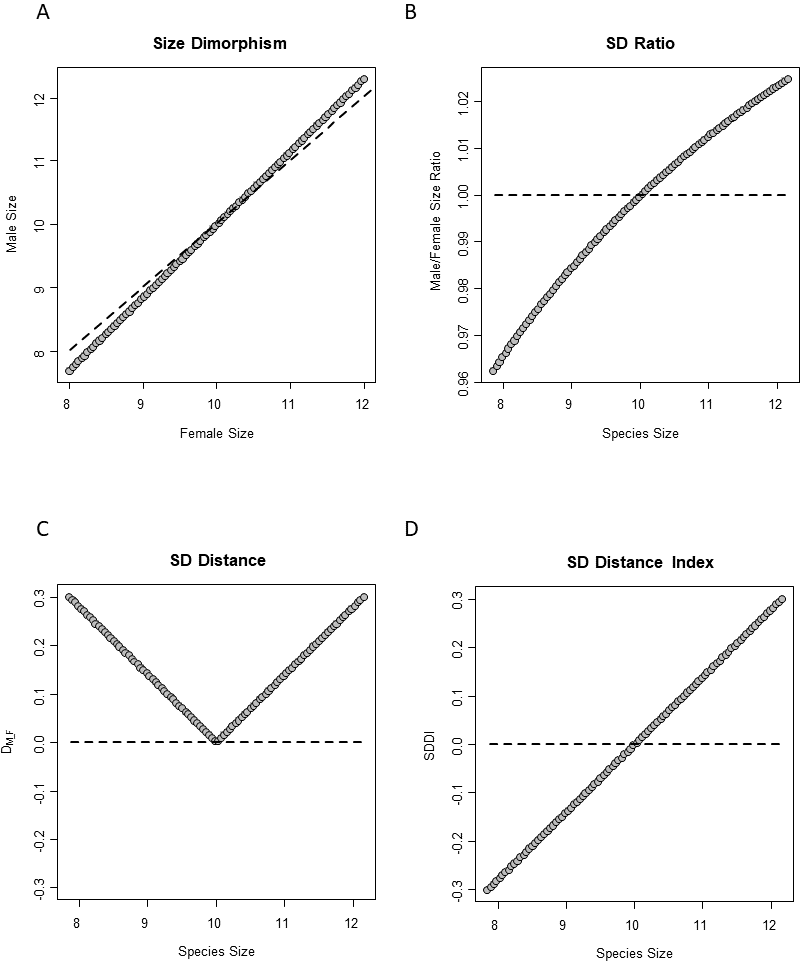
\includegraphics[width=0.95\linewidth]{Fig1}

\singlespacing \textbf{Figure 1}. (A) Sexual size dimorphism for males
and females across 100 hypothetical species. The pattern displayed
exhibits a slope \textgreater{} 1.0, and thus corresponds to Rensch's
rule. (B) The same data represented as the ratio of \(M/F\) sizes
plotted against average species size. (C) Sexual dimorphism represented
as the distance between males and females: \(SDD = D_{M:F}\). (D) Sexual
dimorphism represented as an index of the SD Distance:
\(SDDI = \pm1*D_{M:F}\). In all panels, the dashed line corresponds to
values representing no sexual dimorphism (the 1:1 line). \hfill\break

\newpage

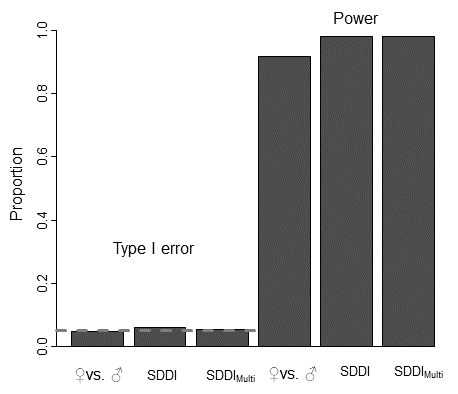
\includegraphics[width=0.7\linewidth]{Fig2}

\singlespacing \textbf{Figure 2}. Results of phylogenetic simulations
testing the type I error and statistical power for detecting patterns
consistent with Rensch's rule. Vertical bars represent the proportion of
datasets found to be significant. For type I error analyses, the dashed
line marks the standard threshold of \(\alpha= 0.05\). For univariate
data, both phylogenetic regression of male versus female size (standard
approach), and \(SDDI\) versus overall body size (new approach) were
performed. For multivariate data, only \(SDDI\) versus overall body size
was examined. \hfill\break

\newpage

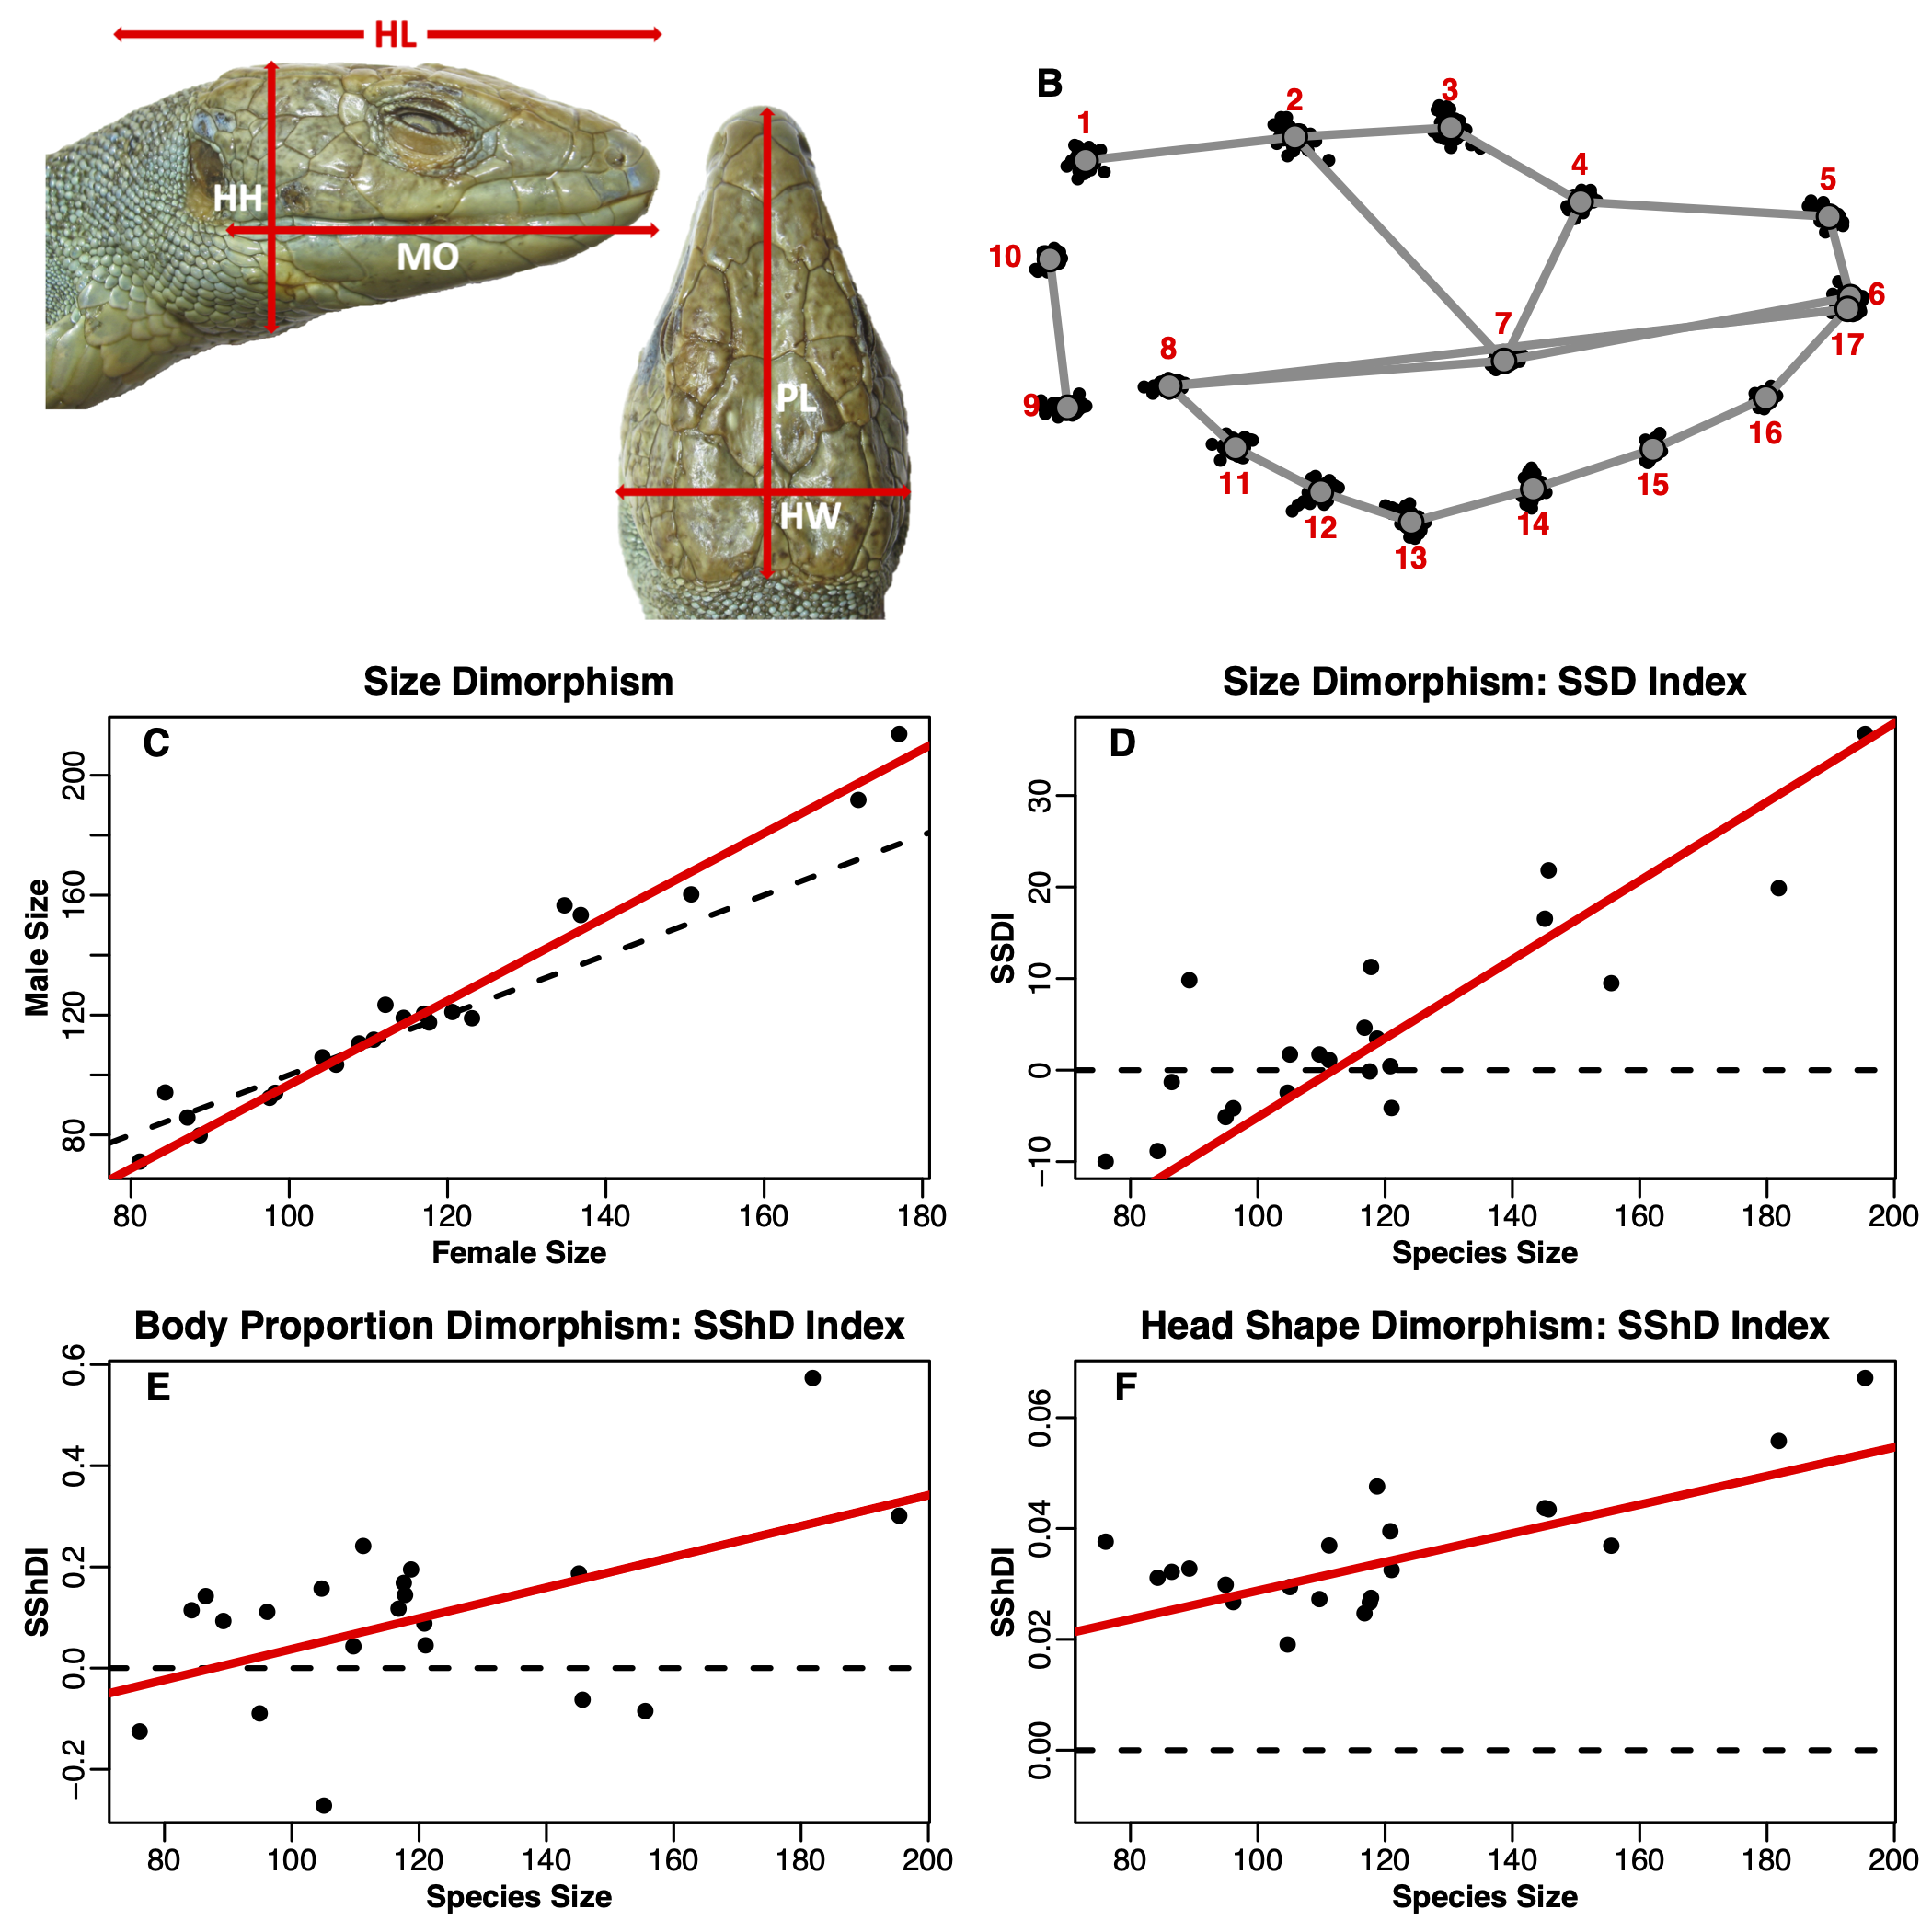
\includegraphics[width=0.95\linewidth]{Fig3}

\singlespacing \textbf{Figure 3}. (A) Set of linear measurements used to
obtain head proportions. HL: head length, HW: head width, HH: head
height, PL: pileus length, MO: mouth opening. (B) Locations of 17
landmarks (1-10; 17) and semilandmarks (11-16) used to quantify head
shape. (C) Patterns of sexual size dimorphism represented as male versus
female size. (D) Patterns of sexual size dimorphism, represented as
sexual size dimorphism index (\(SSDI\)) versus mean size. (E)
Multivariate patterns sexual dimorphism in body proportions (\(SShDI\))
versus mean size. (F) Multivariate patterns of sexual shape dimorphism
(\(SShDI\)) versus mean size. In panels C, D, E, and F, the red line
indicates the regression estimate obtained from the data, while the
dashed line corresponds to values representing no sexual dimorphism.
\hfill\break

\newpage

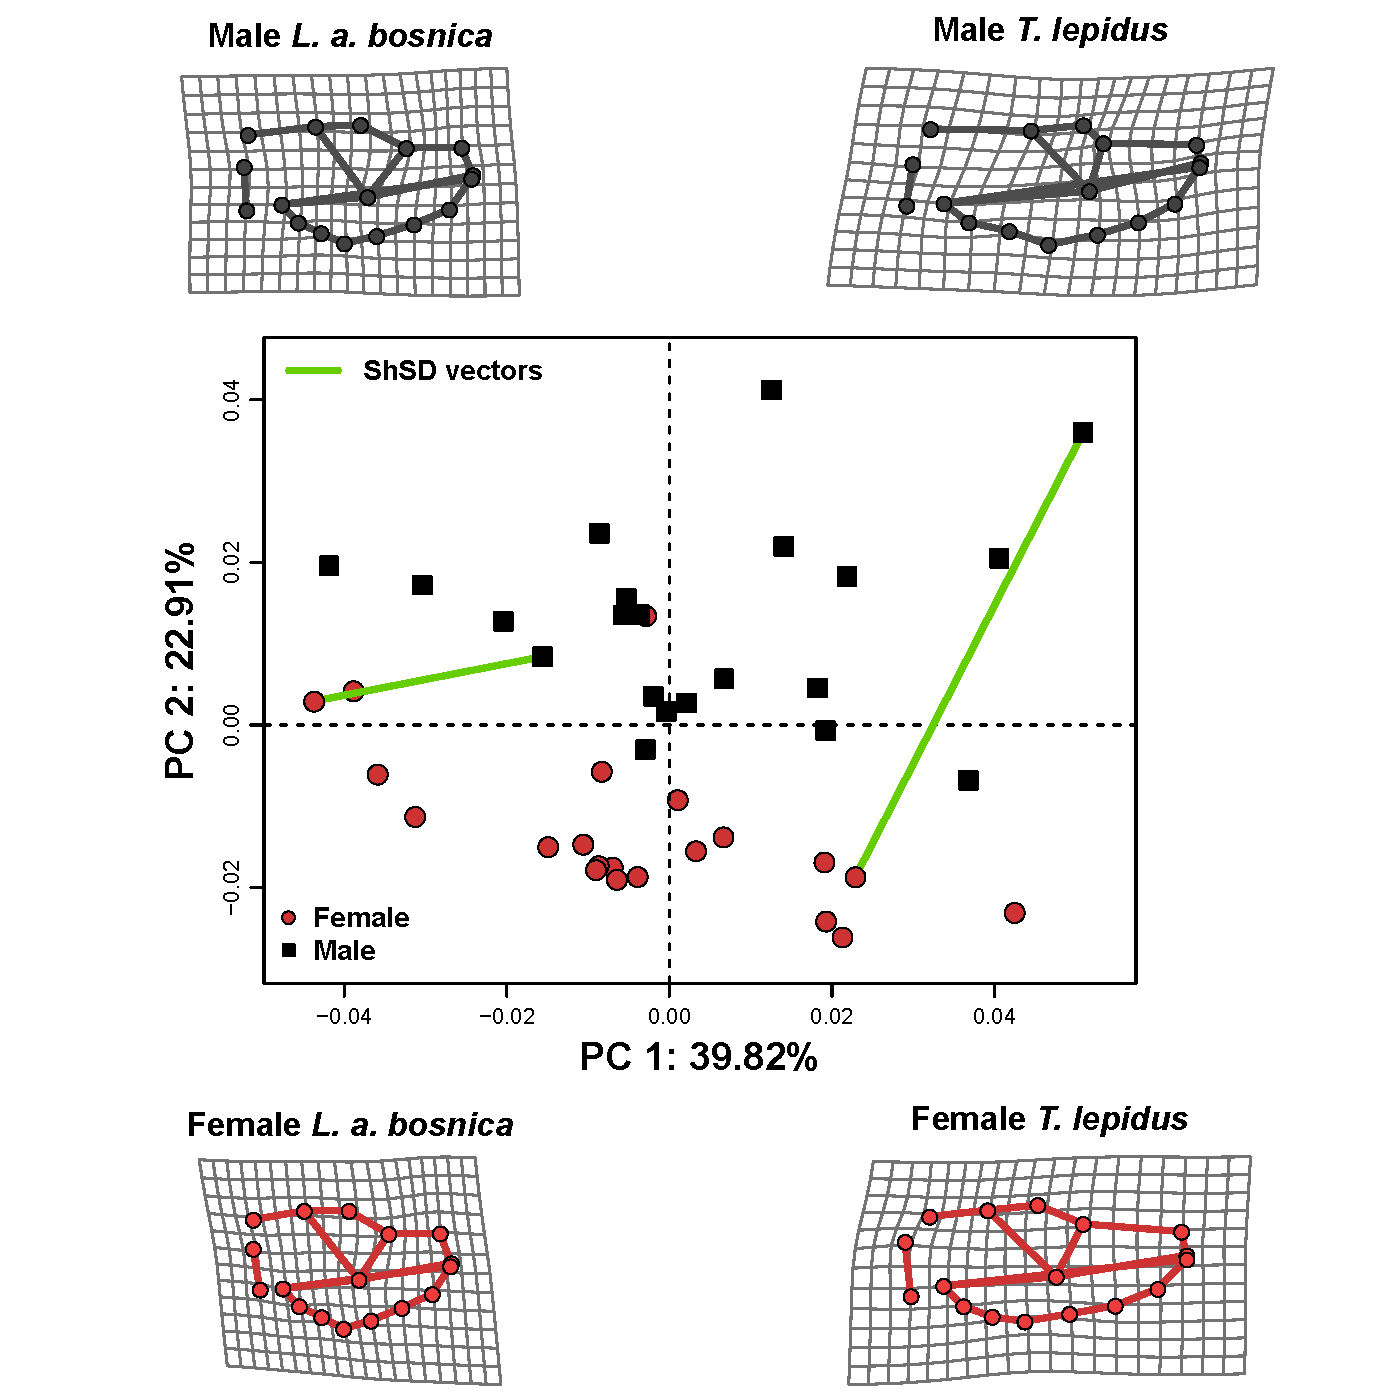
\includegraphics[width=0.95\linewidth]{Fig4}

\singlespacing \textbf{Figure 4}. Principal components plot of male
(black squares) and female (red points) species mean head shape: the
first two PC axes explain over 60\% of the total shape variation. Green
lines correspond to the sexual shape dimorphism in one of the smallest
species, \emph{Lacerta agilis bosnica}, and in the largest species,
\emph{Timon lepidus}. Thin-plate spline deformation grids display the
mean head shape for males and females of these species. \hfill\break

\newpage

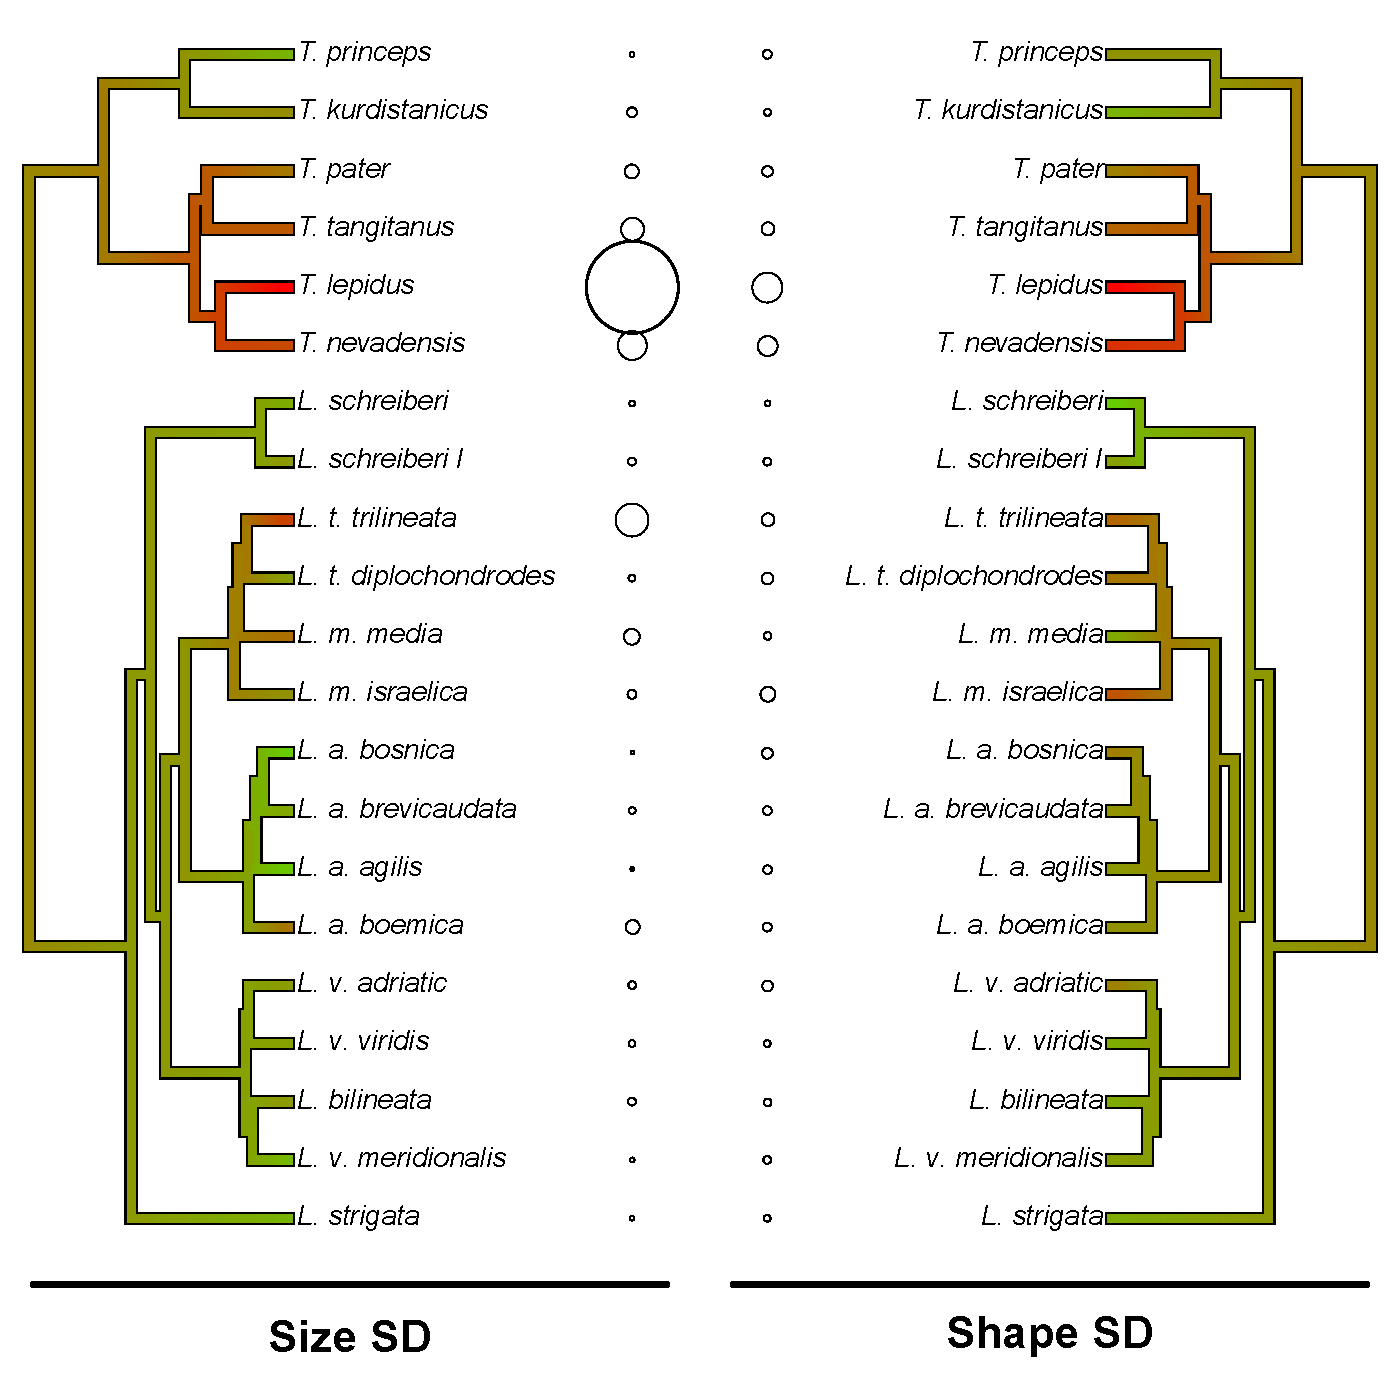
\includegraphics[width=0.95\linewidth]{Fig5}

\singlespacing \textbf{Figure 5}. Heat maps (green: lower values; red:
higher values) displaying the evolution of (A) sexual size dimorphism,
and (B) sexual shape dimorphism across the phylogeny. For each panel, an
index of sexual size dimorphism (\(SSDI\)) or sexual shape dimorphism
(\(SShDI\)) is displayed, with circles being proportional to the degree
of sexual dimorphism. \hfill\break

\end{document}
